\chapter{Technologies Involved} \label{chapter:techonlogies}
This chapter will present the different technologies that make this project possible. It will try to cover the basics for each technology as well as how they function within the context of the project. The following technologies will be covered:
\begin{itemize}
    \item Software Defined Network.
    \item OpenFlow.
    \item Network Slicing Supervisor.
    \item Open vSwitch.
    \item Mininet.
    \item MQTT.
    \item LoRa and LoRaWAN.
\end{itemize}

There are some other, more well known, technologies which will not be covered by this chapter, e.g., operative system virtualization. The reader is expected to be already familiar with such technologies.

\section{Software Defined Network}
Traditionally, each networking device, like a router or a switch, has to be configured individually. This configuration can be done manually, using a script or with the help of configuration tools like NETCONF. In addition, these devices must support a plethora of protocols in order to discover the topology around them (RIP, OSPF, BGP), poll information (SNMP) or support certain configurations (HSRP, GLBP) among other tasks.

As such, each device is expected to have a certain computational strength and, consequently, they require a capable CPU along with an operating system that is able to handle all of the required protocols.

This traditional scenario presents some clear flaws. The major ones are scalability, adaptability and hardware dependency (as the protocols and features supported depend on the hardware used).

This is where Software Defined Networks (SDN) come in, as they were designed to address the flaws and shortcomings of traditional networks. An SDN, at its core, is nothing more than the separation of the control plane and the data plane, shown in Figure \ref{fig:SDN_example}. This means that all of the computational intensive operations are handled by an external entity called \textbf{Controller}, so that the networking device can focus on just forwarding packets and following some simple instructions generated by said controller.

\begin{figure}
  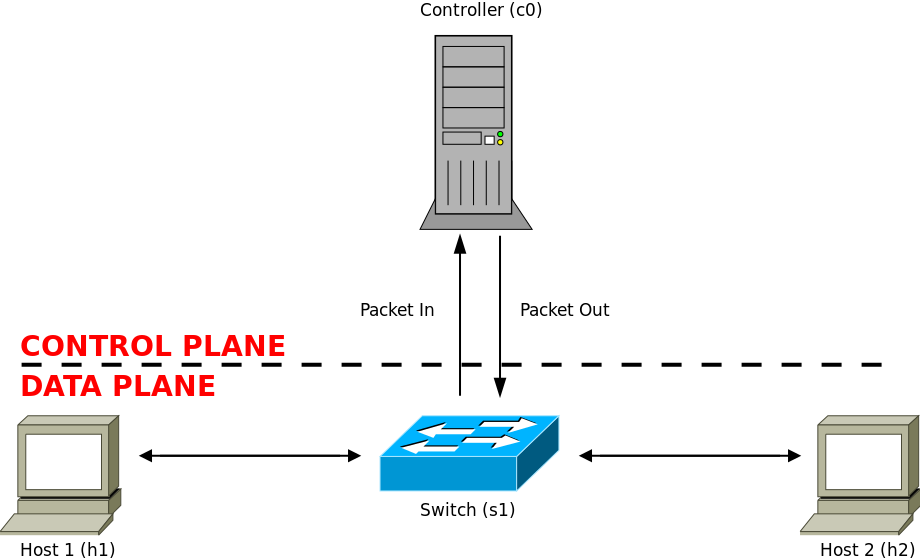
\includegraphics[width=\linewidth]{imagenes/Technologies/SDN.png}
  \caption{Sample SDN topology with a switch as forwarding device.}
  \label{fig:SDN_example}
\end{figure}

In practice, this method has many advantages. Here we list some of them.
\begin{itemize}
    \item \textbf{Cheaper hardware}. The networking devices become just forwarding devices, which do not need to have strong computational capabilities, and hence they can get rely on less powerful CPUs.
    \item \textbf{Global topology vision}. Having a centralized controller allows for a better vision and understanding of the entire network, making tasks such as traffic engineering far simpler.
    \item \textbf{Adaptability}. The controller can quickly reconfigure the forwarding devices if needed.
    \item \textbf{Scalability}. A controller can manage many forwarding devices (although it depends on the services implemented). However, it is possible to increase the number of controllers if necessary. 
    \item \textbf{Hardware agnostic}. Each physical device is just a generic forwarding device, all of the services and protocols are implemented via software on the controller.
\end{itemize}

In general, SDN are a great alternative to traditional networks. They are becoming more and more prevalent as time goes on, and rightfully so. For instance the up and coming 5G mobile technology will be based on this technology.

\section{OpenFlow}
Software Defined Networks and OpenFlow\cite{openflow_specfication} are tightly tied together, since OpenFlow is the communication protocol used between the forwarding devices and the controller or controllers. 

OpenFlow has two main messages, Packet\_In and Packet\_Out. The former, Packet\_In, is used to query the controller when the forwarding device does not know what to do with a certain packet or data stream. The latter, Packet\_Out, is the response to the Packet\_In message. It tells the forwarding device what to do with the packet and, optionally, it might install a flow on that device.

But, what is a flow? A flow is to a forwarding device what an entry in the routing table is to a traditional router. It basically tells the forwarding device what to do with a packet that matches certain fields. A flow has two major components:
\begin{itemize}
    \item \textbf{Matching fields}. As its name indicates, it contains the fields that a packet must match in order to follow this flow.   
    \item \textbf{Action}. What to do with the packet when it matches the flow.
\end{itemize}

A simple example is shown below. This example comes from the tool Open vSwitch, to which section \ref{section_ovswitch} offers a brief overview.
\begin{lstlisting}
    sudo ovs-ofctl add-flow s1 ip,nw_dst=10.0.0.1,actions=output:2
\end{lstlisting}

In this example, we are adding a new flow to a forwarding device called \textbf{s1}. In this flow we are specifying the matching fields as the IP protocol and the destination IP address \textbf{10.0.0.1}, while the action would be to output it through \textbf{port 2} of \textbf{s1}.

An OpenFlow flow supports a wide a variety of matching fields and actions, given the controller a high level of control and granularity over the forwarding devices.

It is also important to note that OpenFlow has several versions that, currently, go from 1.0 to 1.5, with each version mainly adding some new features. Due to technical reasons which will be later discussed, we will be using OpenFlow 1.0 for this project.

\section{Network Slicing Hypervisor}
This is the main element for the project. It is what allows us to slice a physical network into multiple virtual networks. A hypervisor sits between the OpenFlow switches and the controllers, redirecting each Packet\_In to its correspondent controller, as shown in Figure \ref{fig:hypervisor}. This way, a controller only sees a subset of the actual physical network, according to the packages received. Effectively, this is network slicing or virtualization.

If we dive more into the technical details, we find that what a hypervisor actually does, in its simplest form, is create flowspaces. A flowspace is nothing more but a rule or a set of rules that match the incoming packets and assign them to a particular slice.

\begin{figure}
  \centering
  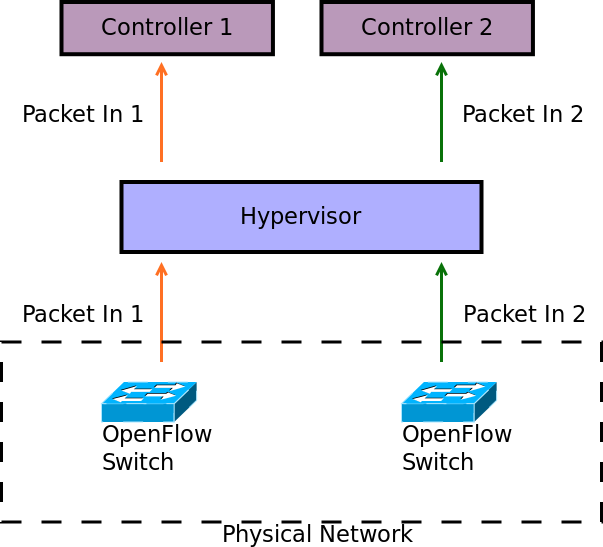
\includegraphics[width=\linewidth]{imagenes/Technologies/hypervisor.png}
  \caption{Simplistic overview of a network virtualization hypervisor.}
  \label{fig:hypervisor}
\end{figure}

In reality the way it works is very similar to just plain OpenFlow. There are rules that match certain packets but, instead of assigning an action to them, a slice is assigned. However, in this case only the Packet\_In are matched against the different rules, as opposed to every packet within the physical network.

Despite its potential usefulness, using a hypervisor also has a few downsides.
\begin{itemize}
    \item \textbf{Single point of failure.} A single hypervisor serves multiple controllers. As a result, a failure in the hypervisor may have extended consequences for several slices, effectively rendering the entire physical network, or a big part of it, unusable.
    
    \item \textbf{Added latency.} The introduction of an extra step for the packets results in a higher delay between the packet arrival and an action being taken. Said delay depends on several factors, e.g., the physical location of the hypervisor and the controllers. This extra delay may not be an issue for most applications, but it might affect the performance of real time applications with strict time constraints.
\end{itemize}

One could also argue that a hypervisor requiring extra configuration is also a downside. However, using a hypervisor usually helps simplify the logic of the controllers that sit above it, therefore reducing the time and cost needed to set up the network.

\section{Open vSwitch} \label{section_ovswitch}
Since we do not have access to physical OpenFlow switches, we have to rely on virtualization. Open vSwitch\cite{ovs_website} (OVS) is a tool that allows us to emulate one or multiple switches which support an ample amount of protocols, such as NetFlow, sFlow, IPFIX, RSPAN, CLI, LACP, 802.1ag, etcetera \cite{ovswitch}.

For the most part, we will not be using OVS directly as it is handled automatically by the the tool in section \ref{Mininet}, Mininet. However, OVS provides a useful command line interface that can prove very useful, especially for debugging, as it allows us to interact directly with the virtual switches. Some of these useful commands are shown below.

\begin{lstlisting}
# Shows the OpenFlow flows installed on a particular virtual switch.
sudo ovs-ofctl dump-flows <switch>
\end{lstlisting}

\begin{lstlisting}
# Useful to map the interface names to their corresponding 
# port number.
sudo ovs-ofctl show <switch>
\end{lstlisting}

\begin{lstlisting}
# Live update of the OpenFlow messages received by the virtual switch.
sudo ovs-ofctl snoop <switch>
\end{lstlisting}

\section{Mininet} \label{Mininet}
On the same topic of virtualization, we may come to the conclusion that virtual switches are not enough to emulate a network. This is the reason why we will use Mininet\cite{mininet_website}, an open source network emulator. While it is possible to do the network emulation manually without the help of Mininet, it would be immensely cumbersome, and thus we opt to use it for its convenience. 

Also, Mininet provides a powerful and easy to use Python API. With this API we can customize the network to our liking, allowing us to control a multitude of variables such as the bandwidth and delay between links, number of hosts, number of switches, number of links between each device, IP addresses, physical addresses and many more.

The power of Mininet resides within some useful features of the Linux kernel such as process groups, CPU bandwidth isolation and network namespaces. These features allow Mininet to produce a lightweight emulation of a small-to-medium size network within a single Linux kernel. In consequence, this is also a limitation, not allowing the hosts to be based on Windows, BSD or any other operating system \cite{mininet}.

Additionally, as we mentioned in section \ref{section_ovswitch}, by default Mininet makes use of Open vSwitch to virtualize the switches. This means that we can take advantage of the Open vSwitch command line interface for debugging and testing purposes.

Although Mininet offers a good amount of features, it does not implement an OpenFlow controller beyond its basic reference controller, meaning we have to implement it ourselves. Thankfully there are several libraries to ease this task like POX (Python) or Beacon (Java), so that it does not become an obstacle when deploying the network.

Lastly, as an example, Figure \ref{fig:mininet_default} shows the default topology created by Mininet, which is two hosts (h1 and h2) connected to one switch (s1) which in turn is connected to the reference controller (c0). The reference controller, albeit very basic, can manage ICMP traffic between the two hosts. This topology happens to be the same as the one shown in Figure \ref{fig:SDN_example}.

\begin{figure}
  \centering
  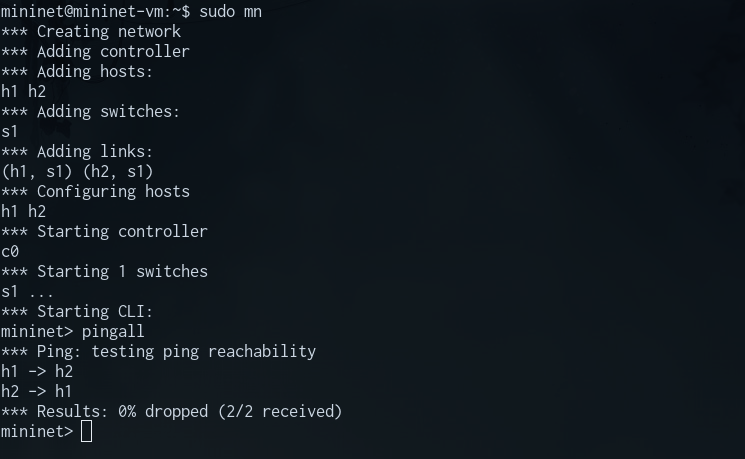
\includegraphics[width=\linewidth]{imagenes/Technologies/mininet_default_topology.png}
  \caption{Default Mininet topology.}
  \label{fig:mininet_default}
\end{figure}

\section{MQTT}
MQTT\cite{mqtt_specfication} was invented in 1999 by Dr Andy Stanford-Clark and can be defined as subscription based connectivity protocol. One of its main strengths is the small bandwidth requirement, it is a very lightweight protocol. Consequently, it makes for an ideal candidate for communications within the IoT environment.

Broadly speaking, the main idea behind MQTT consists on client A subscribing to one ore more topics. When a different client B publishes information under the same topic, it is forwarded to that client A as well as to every other client that is subscribed to that particular topic. In order for this system to work, a third element called \textbf{broker} is placed in between both clients, see Figure \ref{fig:mqtt}. The broker relays each published message to the correspondent subscribers of that topic.

Finally, MQTT spans over different versions, but versions 5.0 and 3.1.1 are of particular importance, as they are OASIS standards.

\begin{figure}
  \centering
  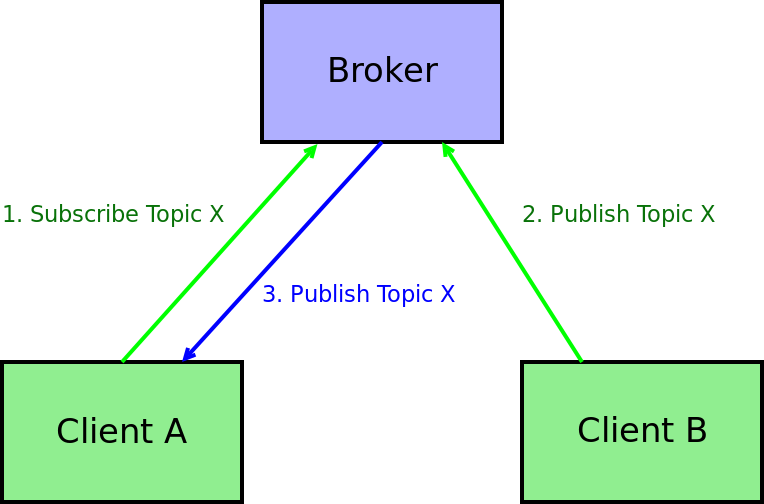
\includegraphics[width=\linewidth]{imagenes/Technologies/mqtt.png}
  \caption{Simplified example of a message transaction using MQTT.}
  \label{fig:mqtt}
\end{figure}

\section{LoRa}
LoRa\cite{lora_website}, currently being developed by Semtech, is a physical layer wireless communication protocol. It is quite a recent technology and it has been growing as a result of the current trend of the Internet of Things.

LoRa is quite a complex technology and it could have its own chapter. Nevertheless, here are, in a very over-simplified way, the main attributes of LoRa.
\begin{itemize}
    \item It relies on the unlicensed Industrial, Scientific and Medical (ISM) band. For example, Europe uses the \SI{868}{\mega\hertz} band while Asia and USA use \SI{433}{\mega\hertz} and \SI{915}{\mega\hertz} respectively. 
    \item Uses a spread spectrum technique based on chirp signals.
    \item Adaptable bandwidth with SNR trade off.
    \item Low power consumption.
    \item Long range communications, emphasized on rural areas. 
    \item Low cost and fairly straightforward to implement.
\end{itemize}

Due to its low power consumption and long range qualities, LoRa fits perfectly as the data communication protocol for IoT devices, especially in rural areas.

\subsection{LoRaWAN}
Tied to LoRa lies LoRaWAN\cite{lorawan}, a Wide Area Network specification based on LoRa. In a LoRaWAN network, there are typically four key components, see Figure \ref{fig:lorawan}.
\begin{itemize}
    \item \textbf{LoRa endpoints}, e.g., sensors. They send data to the network wirelessly through LoRa.
    \item \textbf{Gateway}. Receives the data from the sensors and forwards it, via conventional means (WiFi/Ethernet/Cell network), to the network server.
    \item \textbf{Network server}. Performs some authentication checks and traffic management operations. Eventually sends the data to the application.
    \item \textbf{Application}. Receives the data originally sent by the LoRa endpoint and forwards it to the client that requested it. Typically, this data forwarding is done using MQTT or a REST API.
\end{itemize}

Additionally, LoRaWAN also takes care of Media Access Control (MAC) as well as network security, e.g., authentication and integrity.

\begin{figure}
  \centering
  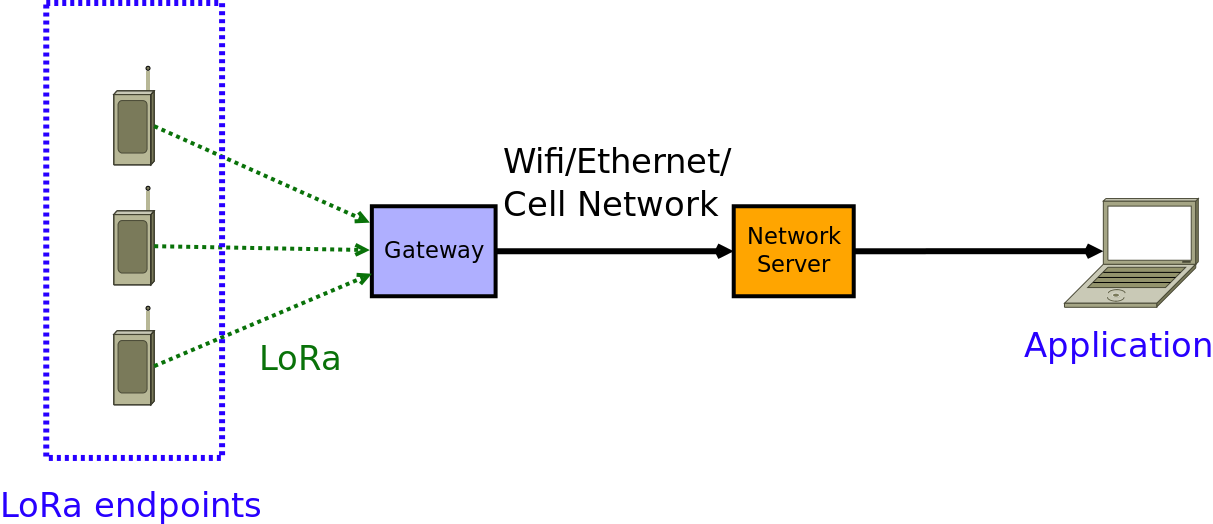
\includegraphics[width=\linewidth]{imagenes/Technologies/lorawan.png}
  \caption{LoRaWAN example network.}
  \label{fig:lorawan}
\end{figure}
